% Evaluation criterion:
%- Language and use of figures
%- Clarity of the problem statement
%- Overall document structure
%- Depth of understanding for the field of computer architecture
%- Depth of understanding of the investigated problem

\section{Introduction}
\label{sec:introduction}
Over the last 3 decades, relative processor performance has increased more than memory performance,
which has led to what is commonly known as the Memory Gap (see figure ~\ref{fig:mem_gap}). In order to remedy this, a memory
hierarchy is used to provide the illusion of a very fast and very
large memory (see figure~\ref{fig:mem_hier}). \cite{tdt4260lect} 

\begin{figure}[H]
	\centering
	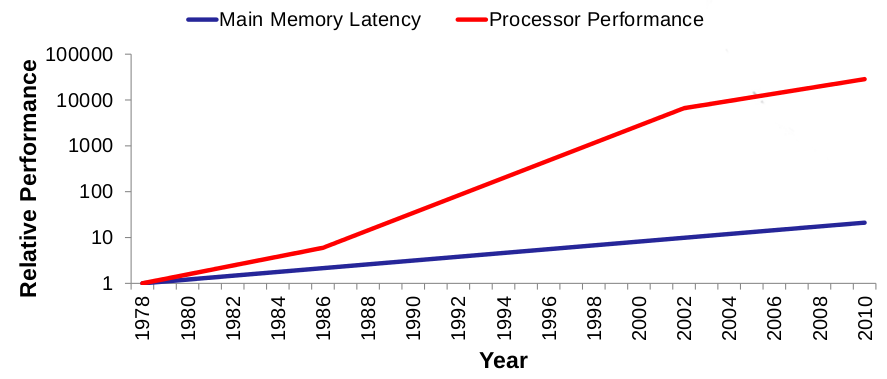
\includegraphics[scale=0.27]{./figures/memwall}
	\caption{The memory gap. Source:\cite{tdt4260lect}}
	\label{fig:mem_gap}
\end{figure}

This illusion will only partially hold, however, as the processor is
delayed for the entire main memory access time when the memory contents required
is not present in any of the caches. One technique
which has been introduced in order to face this problem is prefetching. Prefetching improves the utilization of the caches. This technique
attempts to improve the cache hit rate by predicting what memory
addresses the processor will access in the near future, and
issuing fetches from the main memory before the processor actually
needs the contents so that the data will reside in cache when the
processor requires it. This is usually accomplished by recording
memory access history and statistics, and using this data to make educated
predictions about future memory accesses.\cite{Grannas} 

\begin{figure}[H]
	\centering
	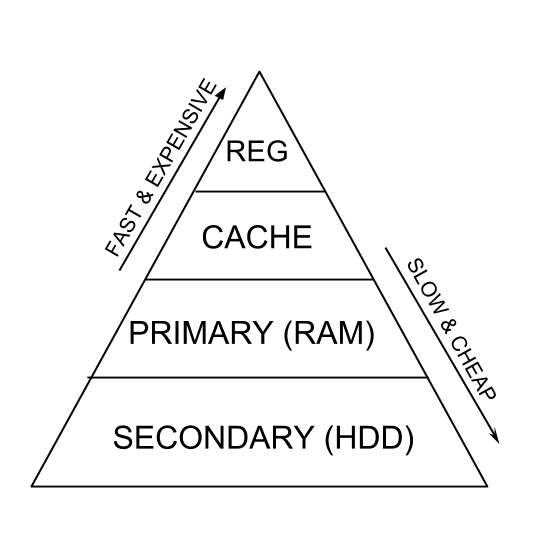
\includegraphics[scale=0.3]{./figures/memhier}
	\caption{The memory hierarchy}
	\label{fig:mem_hier}
\end{figure}

In this paper, we are going to investigate how different kinds of
prefetching strategies performs when run on several different programs from the SPEC CPU2000 benchmark
suite ~\cite{SPECFAQ}.
